\chapter{Návrh přehrávače animace}
\label{section:playerdraft}

V této kapitole je vysvětlen nástroj pro přehrávání animace. Nástroj je vzhledem k~požadavkům vytvořen v~jazyce Javascript.

\section{Vstup}

Vstupem budou dva vytvořené soubory z~generovacího nástroje. Tato aplikace pouze přehrává daný formát, takže je podstatně jednodušší, než generátor animace. 

\section{Návrhový model}

Celá knihovna je díky zjednodušenému přístupu k~jednotlivým elementům  díky knihovně jQuery realizována jako doplněk do této knihovny. Celý návrhový model bude vytvořený tak, aby mohl být doplňkem knihovny jQuery\cite{jqueryplugin}. 


\begin{figure}[h]
\centering
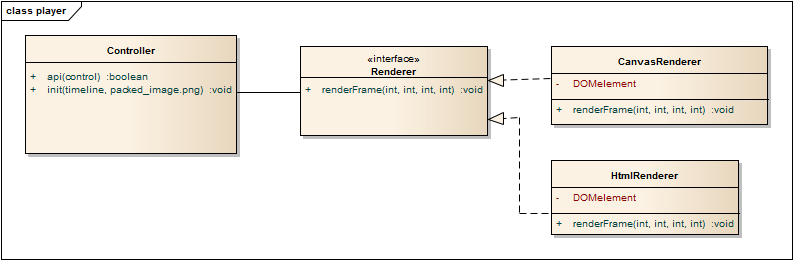
\includegraphics[width=1\textwidth]{figures/player.png}
\caption{Návrhový model knihovny}
\label{fig:player}
\end{figure}


\section{Popis tříd}

Zde je popsán návrhový model tříd knihovny pro přehrávání aplikace. 

\subsection{Controller}
Controller je hlavní třída celé knihovny pro přehrávání, která se stará o~načtení a~přijímá volání přes API. Ze vstupu a~na základě dalších faktorů vybere  správný renderer, který také ovládá. 

\subsection{Renderer}

Renderer je rozhraní, které se stará o~vykreslování animace. Podtřídy tohoto objektu se použijí podle možností prostředí prohlížeče. Na starých prohlížečích, které nepodporují HTML5, je potřeba zajistit zpětnou kompatibilitu (například IE6).

Objekt vykresluje podle souboru s~informacemi bitmapu v~prostředí prohlížeče. 
